\documentclass{beamer}

\usepackage[utf8]{inputenc}
\usepackage{setspace}
\usepackage{amsmath}
\usepackage{amsthm}
\usepackage{amssymb}

\title{T.C.A.S.}
\author[Roberto Bertolini]{Roberto Alessandro Bertolini}
\institute[Liceo Nervi Ferrari]{Liceo "P. Nervi - G. Ferrari" - Morbegno}
\date{Giugno 2021}
\subtitle{Un risolutore di limiti efficiente e compatto}

\usetheme{Warsaw}
\usecolortheme{default}
\usefonttheme{serif}

\begin{document}
	
	\begin{frame}
		\titlepage
	\end{frame}
	
	\begin{frame}
		\frametitle{Indice}
		\tableofcontents
	\end{frame}
	
	\section{Introduzione}
	
	\subsection{La definizione di limite}
	\begin{frame}
		\frametitle{La definizione di limite}
		\begin{block}{Definizione di limite di una funzione}
			\[ 
			\lim_{x \to x_{0}}{f(x) = l} 
			\]
			
			Se \( 
			\forall \varepsilon > 0 \enspace \exists \enspace \delta(\varepsilon) \mid \forall x \in D_{f}, 0 < \: \mid x - x_{0} \mid \: <\delta \implies \mid f(x) - l \mid < \varepsilon
			\)
		\end{block}
		
	\end{frame}
	
	\subsection{La risoluzione per approssimazione}
	\begin{frame}
		\frametitle{La risoluzione per approssimazione}
		\begin{columns}
			\begin{column}{0.5\textwidth}
				Consideriamo \(
					f(x) = \frac{1}{x^{\ln{\ln{\ln{\ln{\frac{1}{x}}}}}-1}}
				\)
				
				\vspace{5mm}
				\onslide<2-7>{Cerchiamo \(\lim_{x \to 0^{+}}{f(x)}\)}
				
				\onslide<8->{Cerchiamo \(\lim_{x \to 0^{+}}{f(x)} = 0\)}
				
				\vspace{5mm}
				\onslide<8->{
					Eppure \(\lim_{x \to 0^{+}}{f(x)} = +\infty\)
				}
			
				\vspace{5mm}
				\onslide<9>{
					La funzione ha un minimo in \(x \approx 4.29 \times 10 ^{-1656521}\)
				}
			
			\end{column}
			\begin{column}{0.5\textwidth}
				\begin{figure}
					\begin{overprint}
						\onslide<2>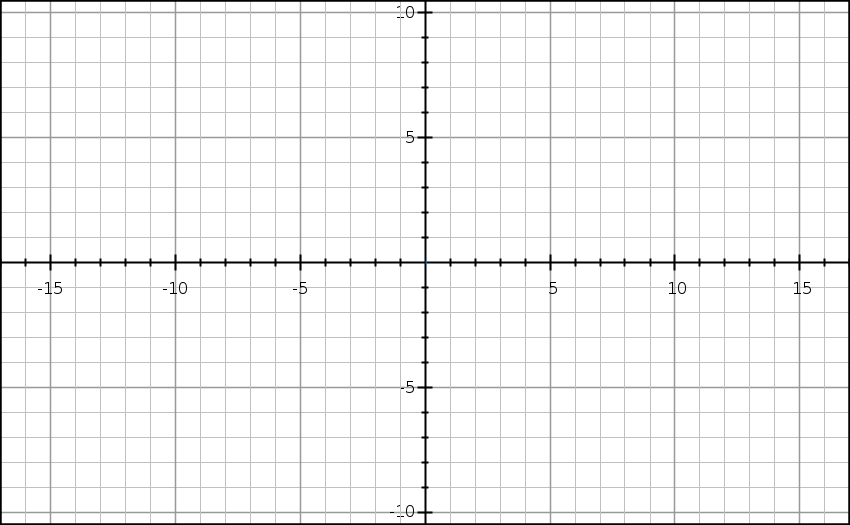
\includegraphics[width=\textwidth]{pres_img/f1.png}
						\onslide<3>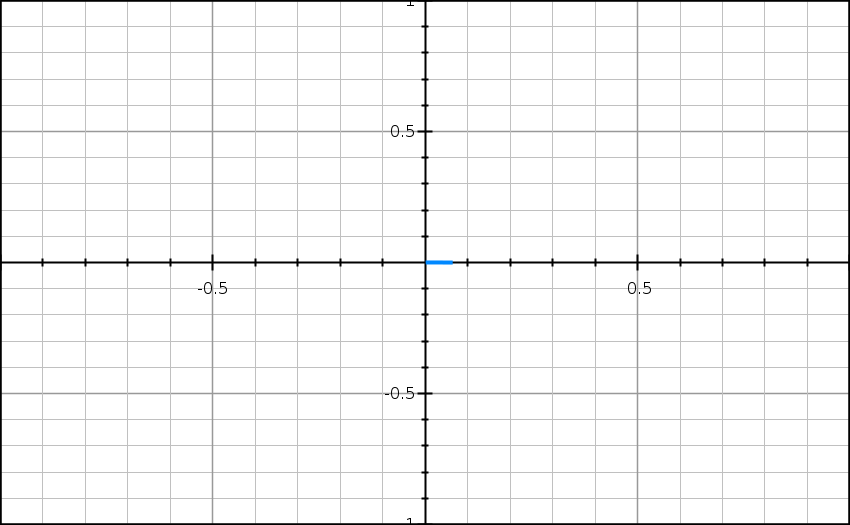
\includegraphics[width=\textwidth]{pres_img/f2.png}
						\onslide<4>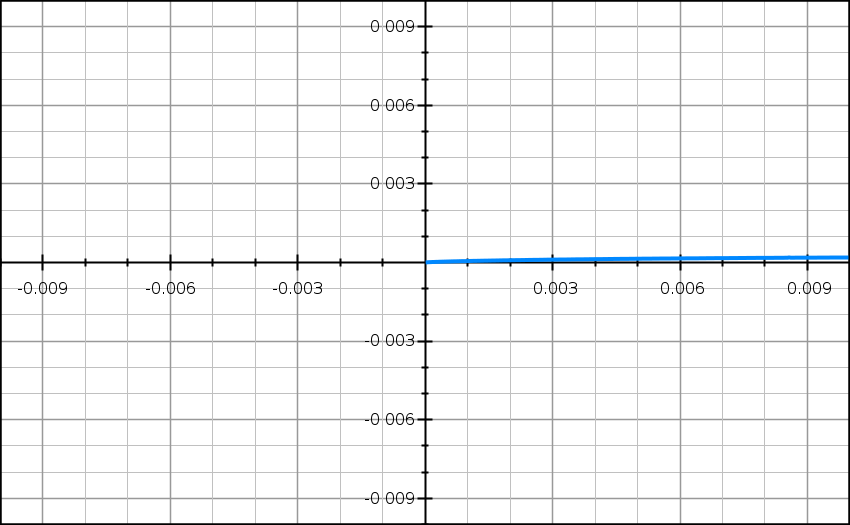
\includegraphics[width=\textwidth]{pres_img/f3.png}
						\onslide<5>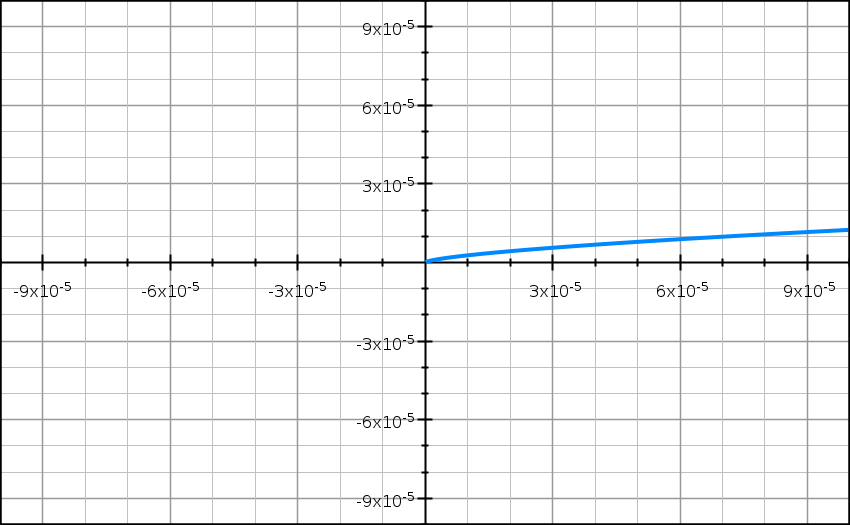
\includegraphics[width=\textwidth]{pres_img/f4.png}
						\onslide<6>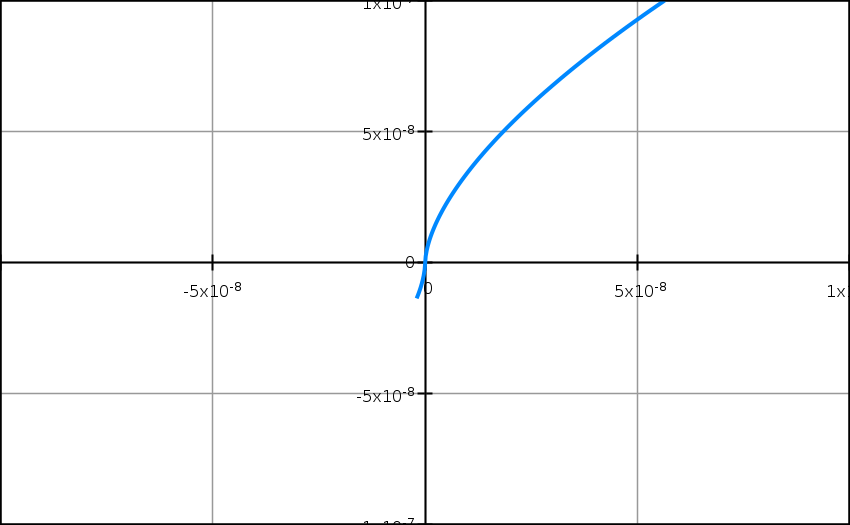
\includegraphics[width=\textwidth]{pres_img/f5.png}
						\onslide<7->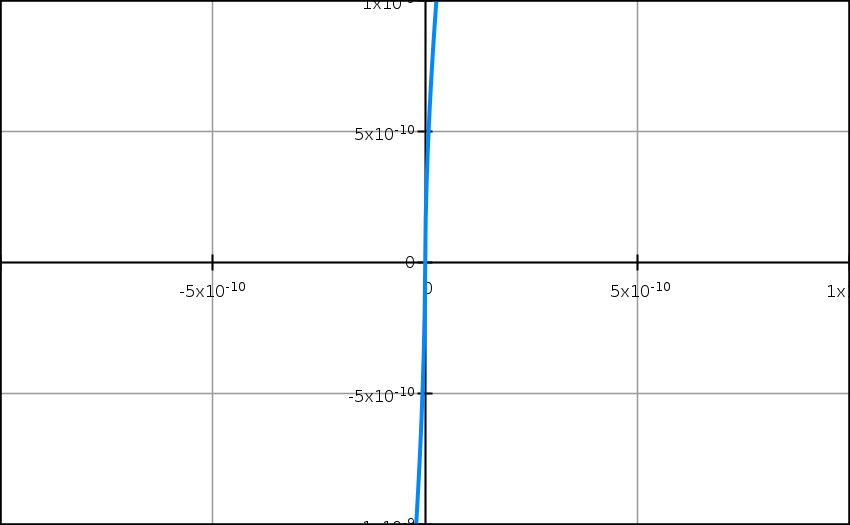
\includegraphics[width=\textwidth]{pres_img/f6.png}
					\end{overprint}
				\end{figure}
			\end{column}
		\end{columns}
	\end{frame}
	
	\subsection{L'approccio matematico}
	\begin{frame}
		\frametitle{L'approccio matematico}
		\begin{block}{La regola di De L'Hôpital}
			\[
			\begin{aligned}
				\text{Se} &\lim_{x \to x_{0}}{f(x)} = \lim_{x \to x_{0}}{g(x)} = 0 \\ \text{oppure} &\lim_{x \to x_{0}}{\lvert f(x) \rvert} = \lim_{x \to x_{0}}{\lvert g(x) \rvert} = \infty \\ \text{ed esiste} &\lim_{x \to x_{0}}{\frac{f'(x)}{g'(x)}} = l \in \mathbf{R} \\ \text{allora} &\lim_{x \to x_{0}}{\frac{f(x)}{g(x)}} = l
			\end{aligned}
			\]
		\end{block}
	\end{frame}
	
	\section{TCAS}
	
	\subsection{Il parsing dell'espressione}
	\begin{frame}
		\frametitle{Il parsing dell'espressione}
	\end{frame}
	
	
	
\end{document}